\section{Darwinia ChainRelay Applications}

Here we need to briefly introduce the characteristics of our products

\subsection*{Token Bridge}

The cross-chain token bridge refers to the asset transfer channel between two heterogeneous chains. Through the token bridge, assets can be safely and reliably transferred on different heterogeneous chains. The subsequent token bridge solution in this article will be backed by the concept of cryptocurrency backed asset(CBA) model and decentralized backing technology.

\subsubsection*{Cryptocurrency Backed Asset Model(CBA Model)}

To describe the solution more accurately and clearly, we use the cryptocurrency backed asset (CBA) model to describe it. In the cross-chain CBA model, two heterogeneous chains are called backing blockchain and issuing blockchain. Cross-chain assets do not exist natively on both chains, but through backing technology, by locking as backing assets on the backing chain, while issuing assets on the issuing chain for cross-chain circulation. The assets issued by backing native assets on the backing blockchain are called backed assets, or CBA for short. The security and redeemability of backed assets are determined by the security and reliability of decentralized backing technology.

Darwinia cross-chain token bridge is a cross-chain bridge solution between the backing chain and the issuing chain, and it is also a decentralized asset backing technology.

    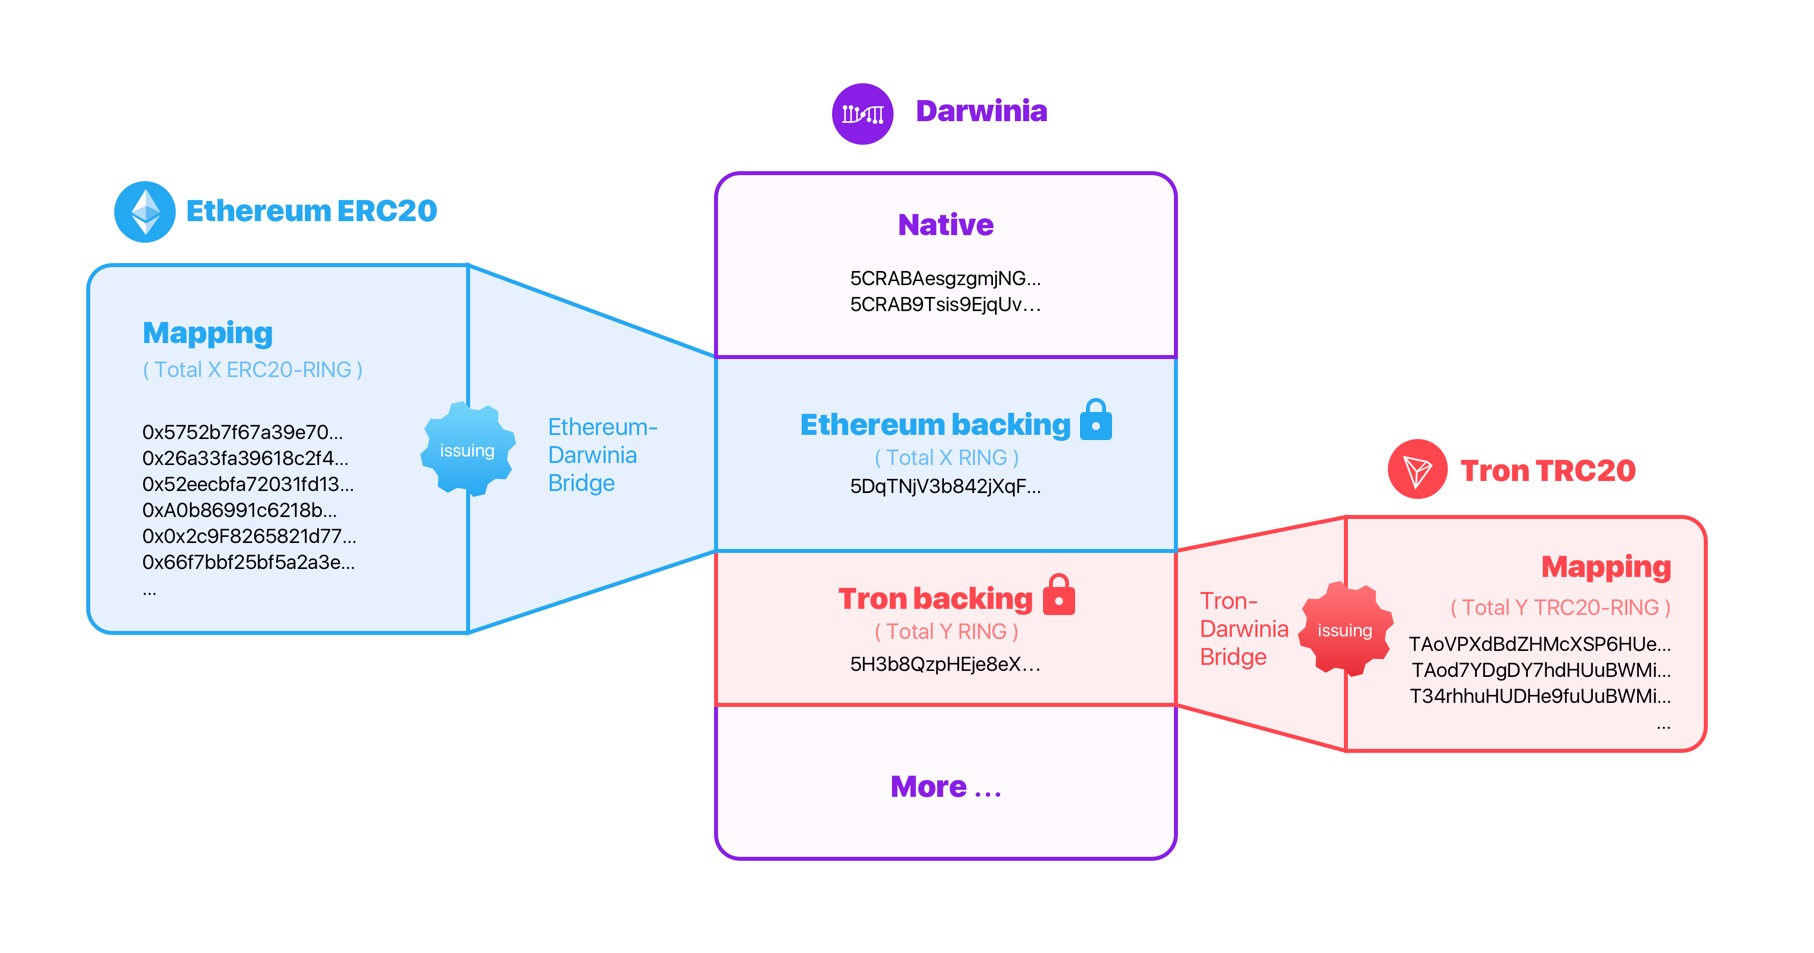
\includegraphics[scale=0.12]{pic/tokenbank.jpg}


\subsubsection*{Decentralized Backing Technology}

Decentralized backing technology is a more accurate description of cross-chain asset gateway technology, which mainly includes cross-chain verification modules and backed issuing modules. In the case of not strictly distinguishing the degree of centralization, the backing method also includes the traditional centralized backing method, for example, a method operated by an external institution, such as USDT, the backing asset is USD, and CBA is USDT issued on other chains.

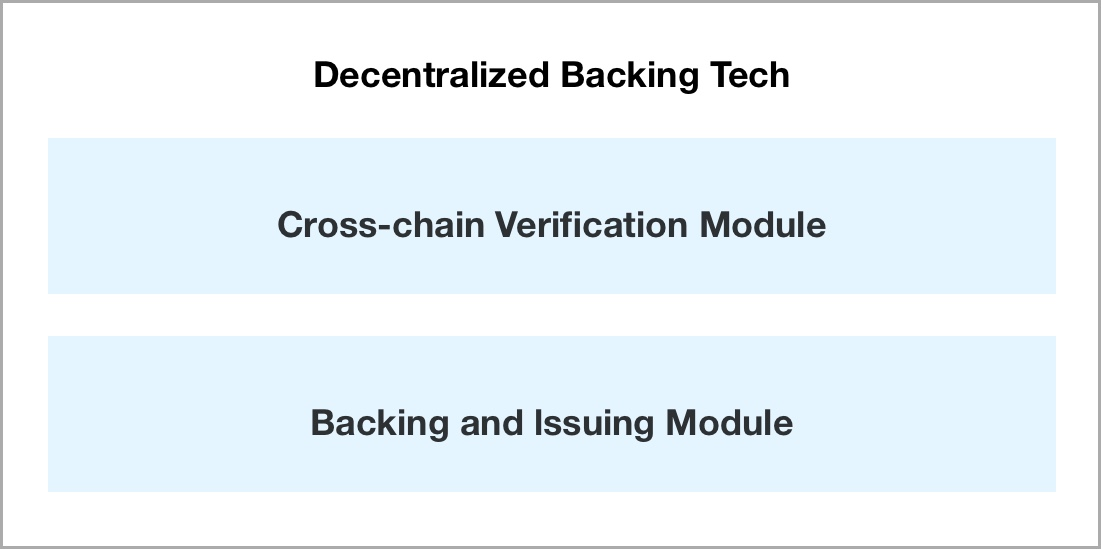
\includegraphics[scale=0.2]{pic/Decentralized Backing Technology.jpg}

Common decentralized backing techniques include:

\begin{itemize}
    \item There are trust nodes or custodian mechanisms, where the trusted node or custodian uses multi-signature / threshold signature and other multi-centralized technologies to avoid single points of failure, such as Parity Bridge, ChainX, etc.
    \item Some solutions use collateralized bridges to ensure the redeemability of cross-chain assets, partially combined with Chain Relay.  XClaim has the disadvantage that it is only suitable for homogeneous assets with good liquidity, and its economic feasibility is relatively weak.
    \item Fully use the Chain Relay for chain verification, such as BTCRelay, WaterLoo, Darwinia ChainRelay, etc. The prerequisite of using this solution is that the issuing chain needs to support the implementation of smart contracts, on-chain runtimes, hard forks, and other methods. Such blockchains like Chain Relay and  Bitcoin network cannot be used as an issuing chain. The advantage is that it can support a variety of native assets, including illiquid assets and NFT assets. Economic feasibility depends on the type of Chain Relay. Sub-linear Chain Relay can achieve better economic feasibility.

\end{itemize}

\subsection*{Darwinia Cross-chain Token Bridge}


Darwinia's cross-chain token bridge solution is a two-way cross-chain token bridge based on chain relay. The chain relay we are going to develop adopts the design of the Darwinia Sublinear Relay, which has better performance and economic feasibility.

\begin{figure*}
\centering
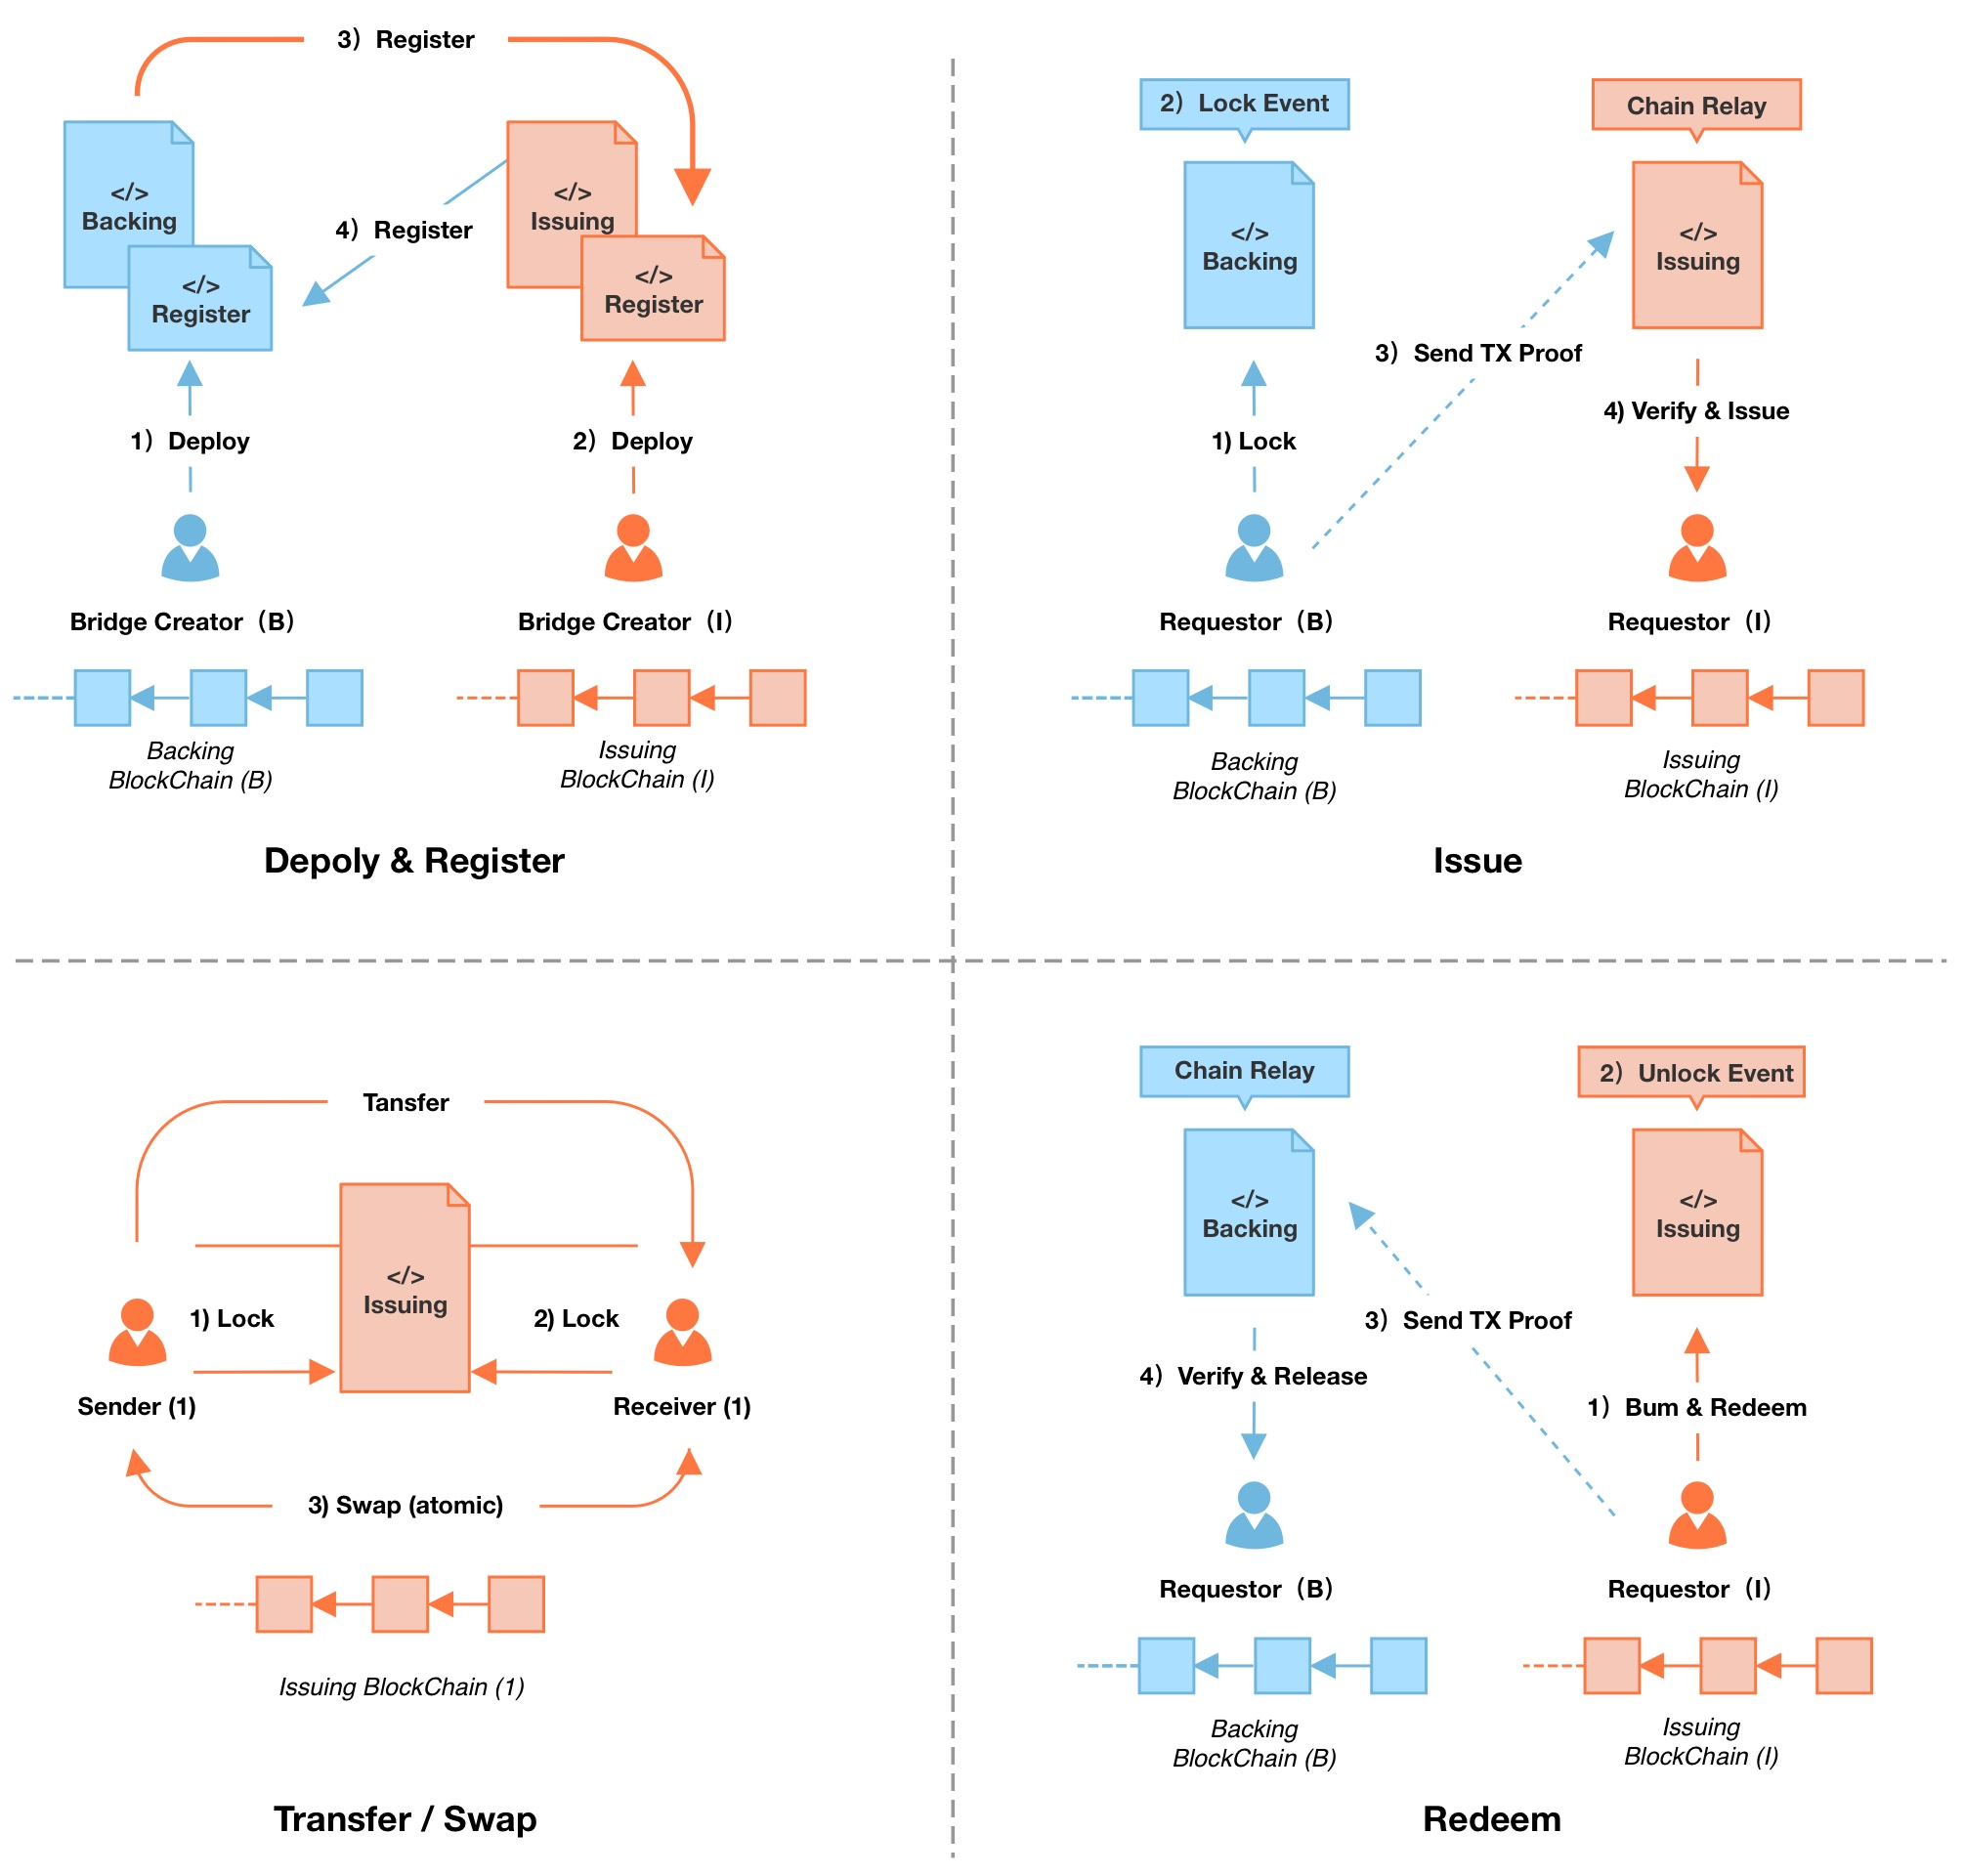
\includegraphics[scale=0.2]{pic/High-Level Protocol Overview.jpg}
\caption{High-Level Protocol Overview}
\label{fig:picture001}
\end{figure*}

\begin{figure*}
\centering
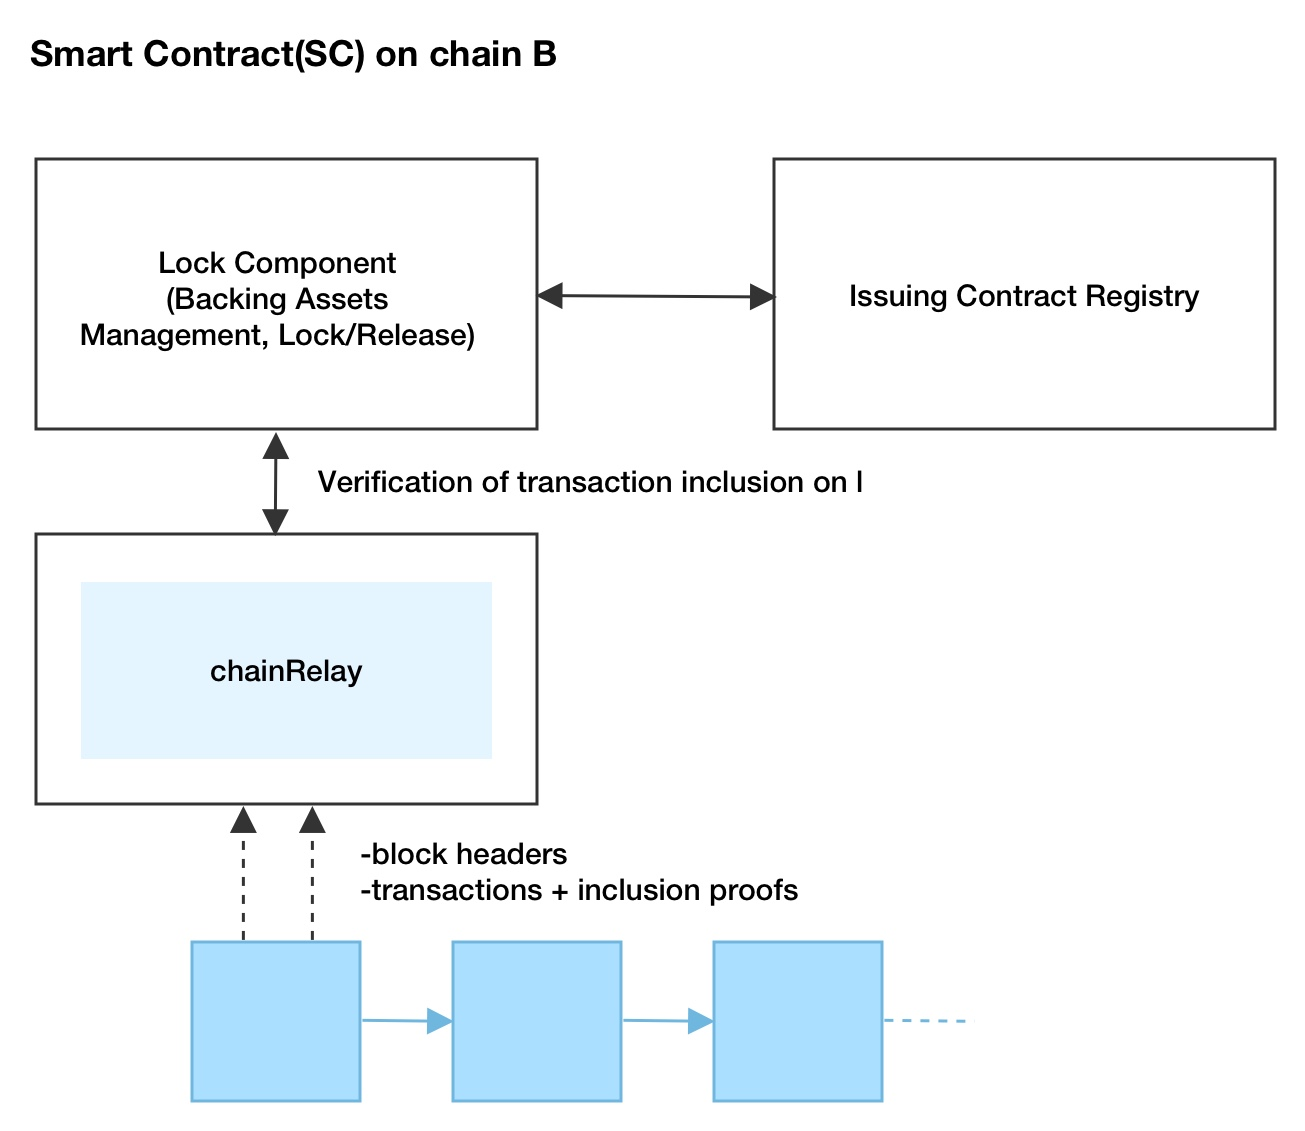
\includegraphics[scale=0.2]{pic/Smart Contract(SC) on chain B.jpg}
\caption{Composition of cross-chain token bridge module on backing chain}
\label{fig:picture001}
\end{figure*}

\subsection*{}

\begin{figure*}
\centering
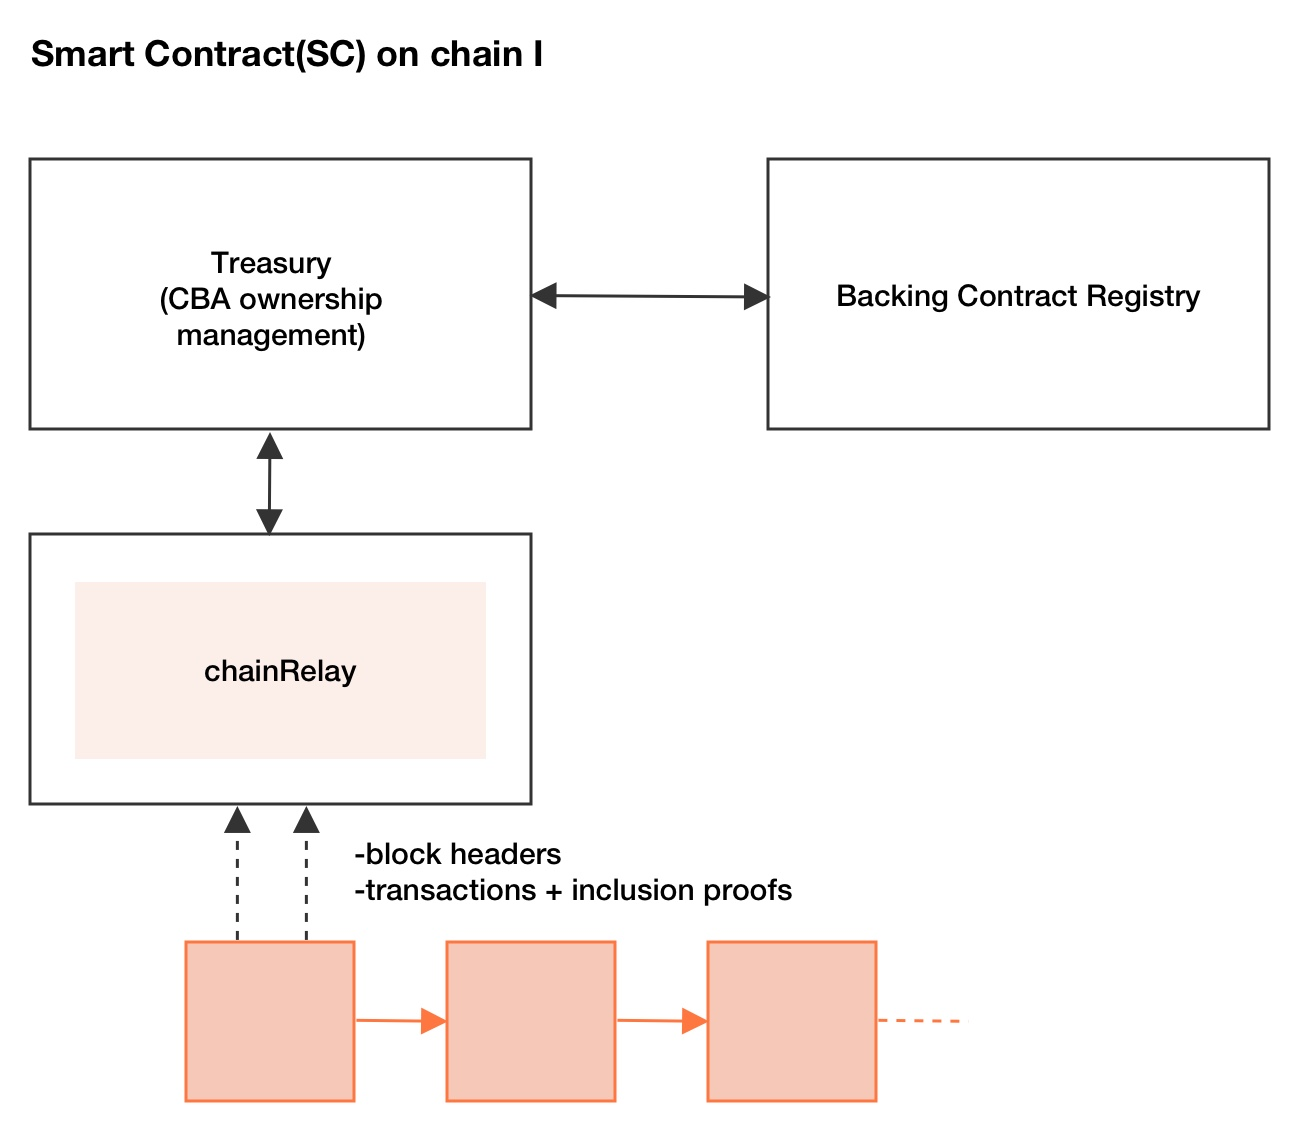
\includegraphics[scale=0.2]{pic/Smart Contract(SC) on chain I.jpg}
\caption{Composition of cross-chain transfer bridge modules on the issuing chain}
\label{fig:picture001}
\end{figure*}

\newpage